% Some commands used in this file
\newcommand{\package}{\emph}

\chapter{Introduction}

\pengcheng{Concept of smartnic}
In recent years, the scaling potential of CPU-based networking stacks capacity gradually slowdowns compared to the NIC links due to hurdles of Moore's law scaling. SmartNIC is an emerging approach to increase networking throughput and reduce packet processing latency by combining compute cores with traditional NIC functionality. Existing SmartNIC architectures could be generally classified into two categories. The \textit{bump-in-the-wire} architecture comprises wimpy energy-efficient programmable cores placed within the NIC packet datapath. The \textit{side-band} architectures feature the SoC running a fully-fledged OS (e.g., Linux) that sees the NIC interface as a PCIe device.

A typical use-case of a SmartNIC is offloading the parts of user application that could be entirely done \textit{in the network}, e.g., gradient averaging in distributed deep learning. Thus, similarly to GPUs, SmartNICs need a hardware/software stack that could linearly scale with the data-arrival rates, a convenient API, and a management infrastructure that allows the users to benefit from in-network computing at the cost of \textit{minimal} changes to the application.

This project is a full end-to-end system demo of \underline{F}PGA-based \underline{PsPIN} SmartNIC~\cite{di2021risc} designed with a bump-in-the-wire architecture. We present the open-source hardware-software SmartNIC stack prototype capable of offloading various I/O and compute parts of the user applications using the sPIN programming model. We explain the hardware and software design of the FPsPIN system and showcase preliminary performance results in two real-world demo applications. While still a work in progress, the project already demonstrates the promising capabilities of sPIN-based SmartNIC in real life.

\begin{figure}
    \centering
    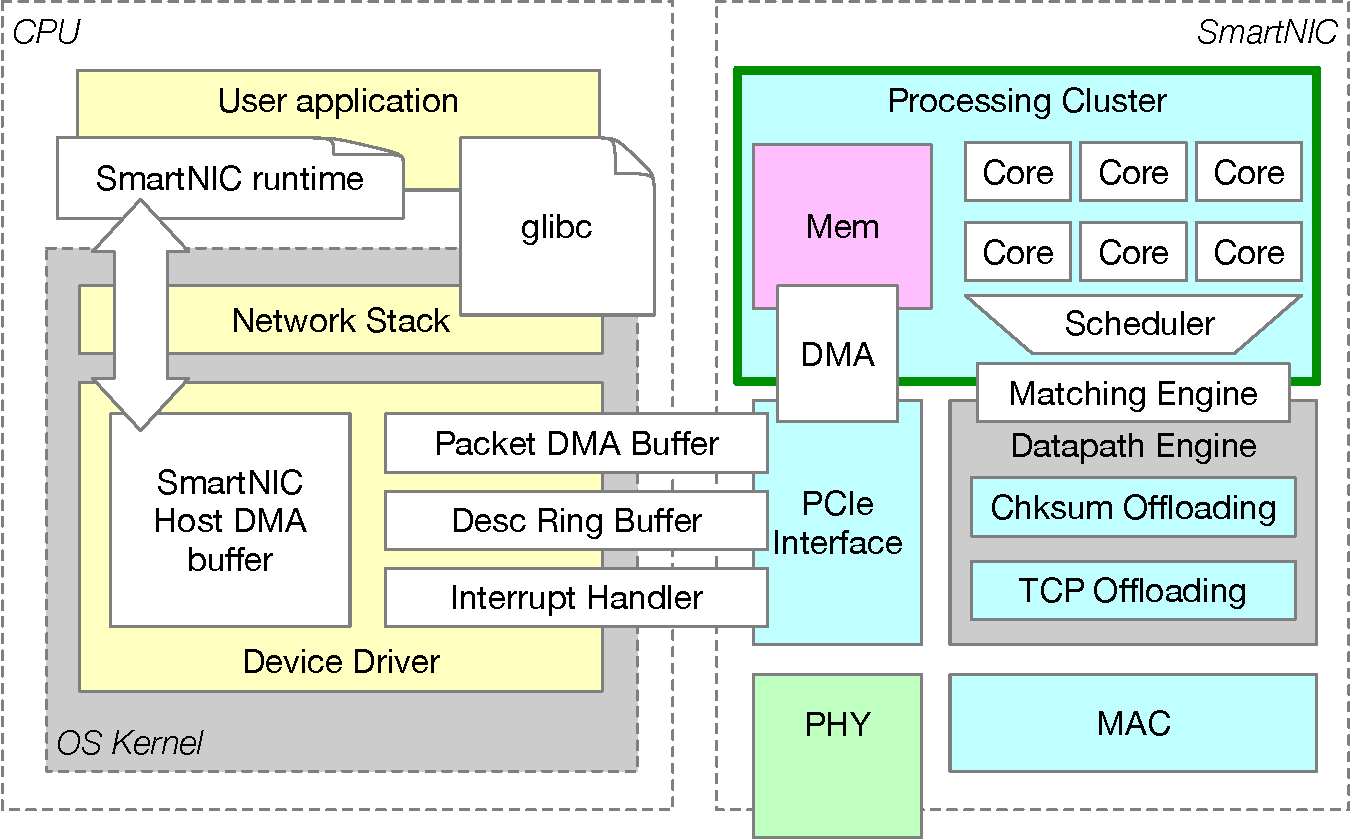
\includegraphics[width=.9\linewidth]{figures/system-overview.pdf}
    \caption{Overview of the complete server system, showing the software stack on the CPU and hardware components on the SmartNIC.  The green box marks the existing PsPIN processing cluster available from previous work.  Everything else needs to be developed, integrated and tested.}
    \label{fig:full-system}
\end{figure}